\chapter{Результаты экспериментов}

\section{Детальные результаты экспериментов}

В данном приложении представлены детальные результаты всех проведенных экспериментов.

\subsection{Эксперимент 1: Базовое тестирование}

\begin{table}[H]
\centering
\caption{Детальные результаты эксперимента 1}
\begin{tabular}{|l|c|c|c|c|}
\hline
№ & Параметр 1 & Параметр 2 & Параметр 3 & Результат \\
\hline
1 & 0.1 & 0.2 & 0.3 & 0.95 \\
2 & 0.2 & 0.3 & 0.4 & 0.87 \\
3 & 0.3 & 0.4 & 0.5 & 0.92 \\
\hline
\end{tabular}
\label{tab:detailed_exp1}
\end{table}

\subsection{Эксперимент 2: Сравнительное тестирование}

\begin{table}[H]
\centering
\caption{Сравнительные результаты}
\begin{tabular}{|l|c|c|c|}
\hline
Метод & Точность & Время (с) & Память (МБ) \\
\hline
Метод 1 & 0.95 & 1.2 & 128 \\
Метод 2 & 0.87 & 0.8 & 96 \\
Наш метод & 0.98 & 1.0 & 112 \\
\hline
\end{tabular}
\label{tab:comparison}
\end{table}

\section{Дополнительные графики}

\begin{figure}[H]
\centering
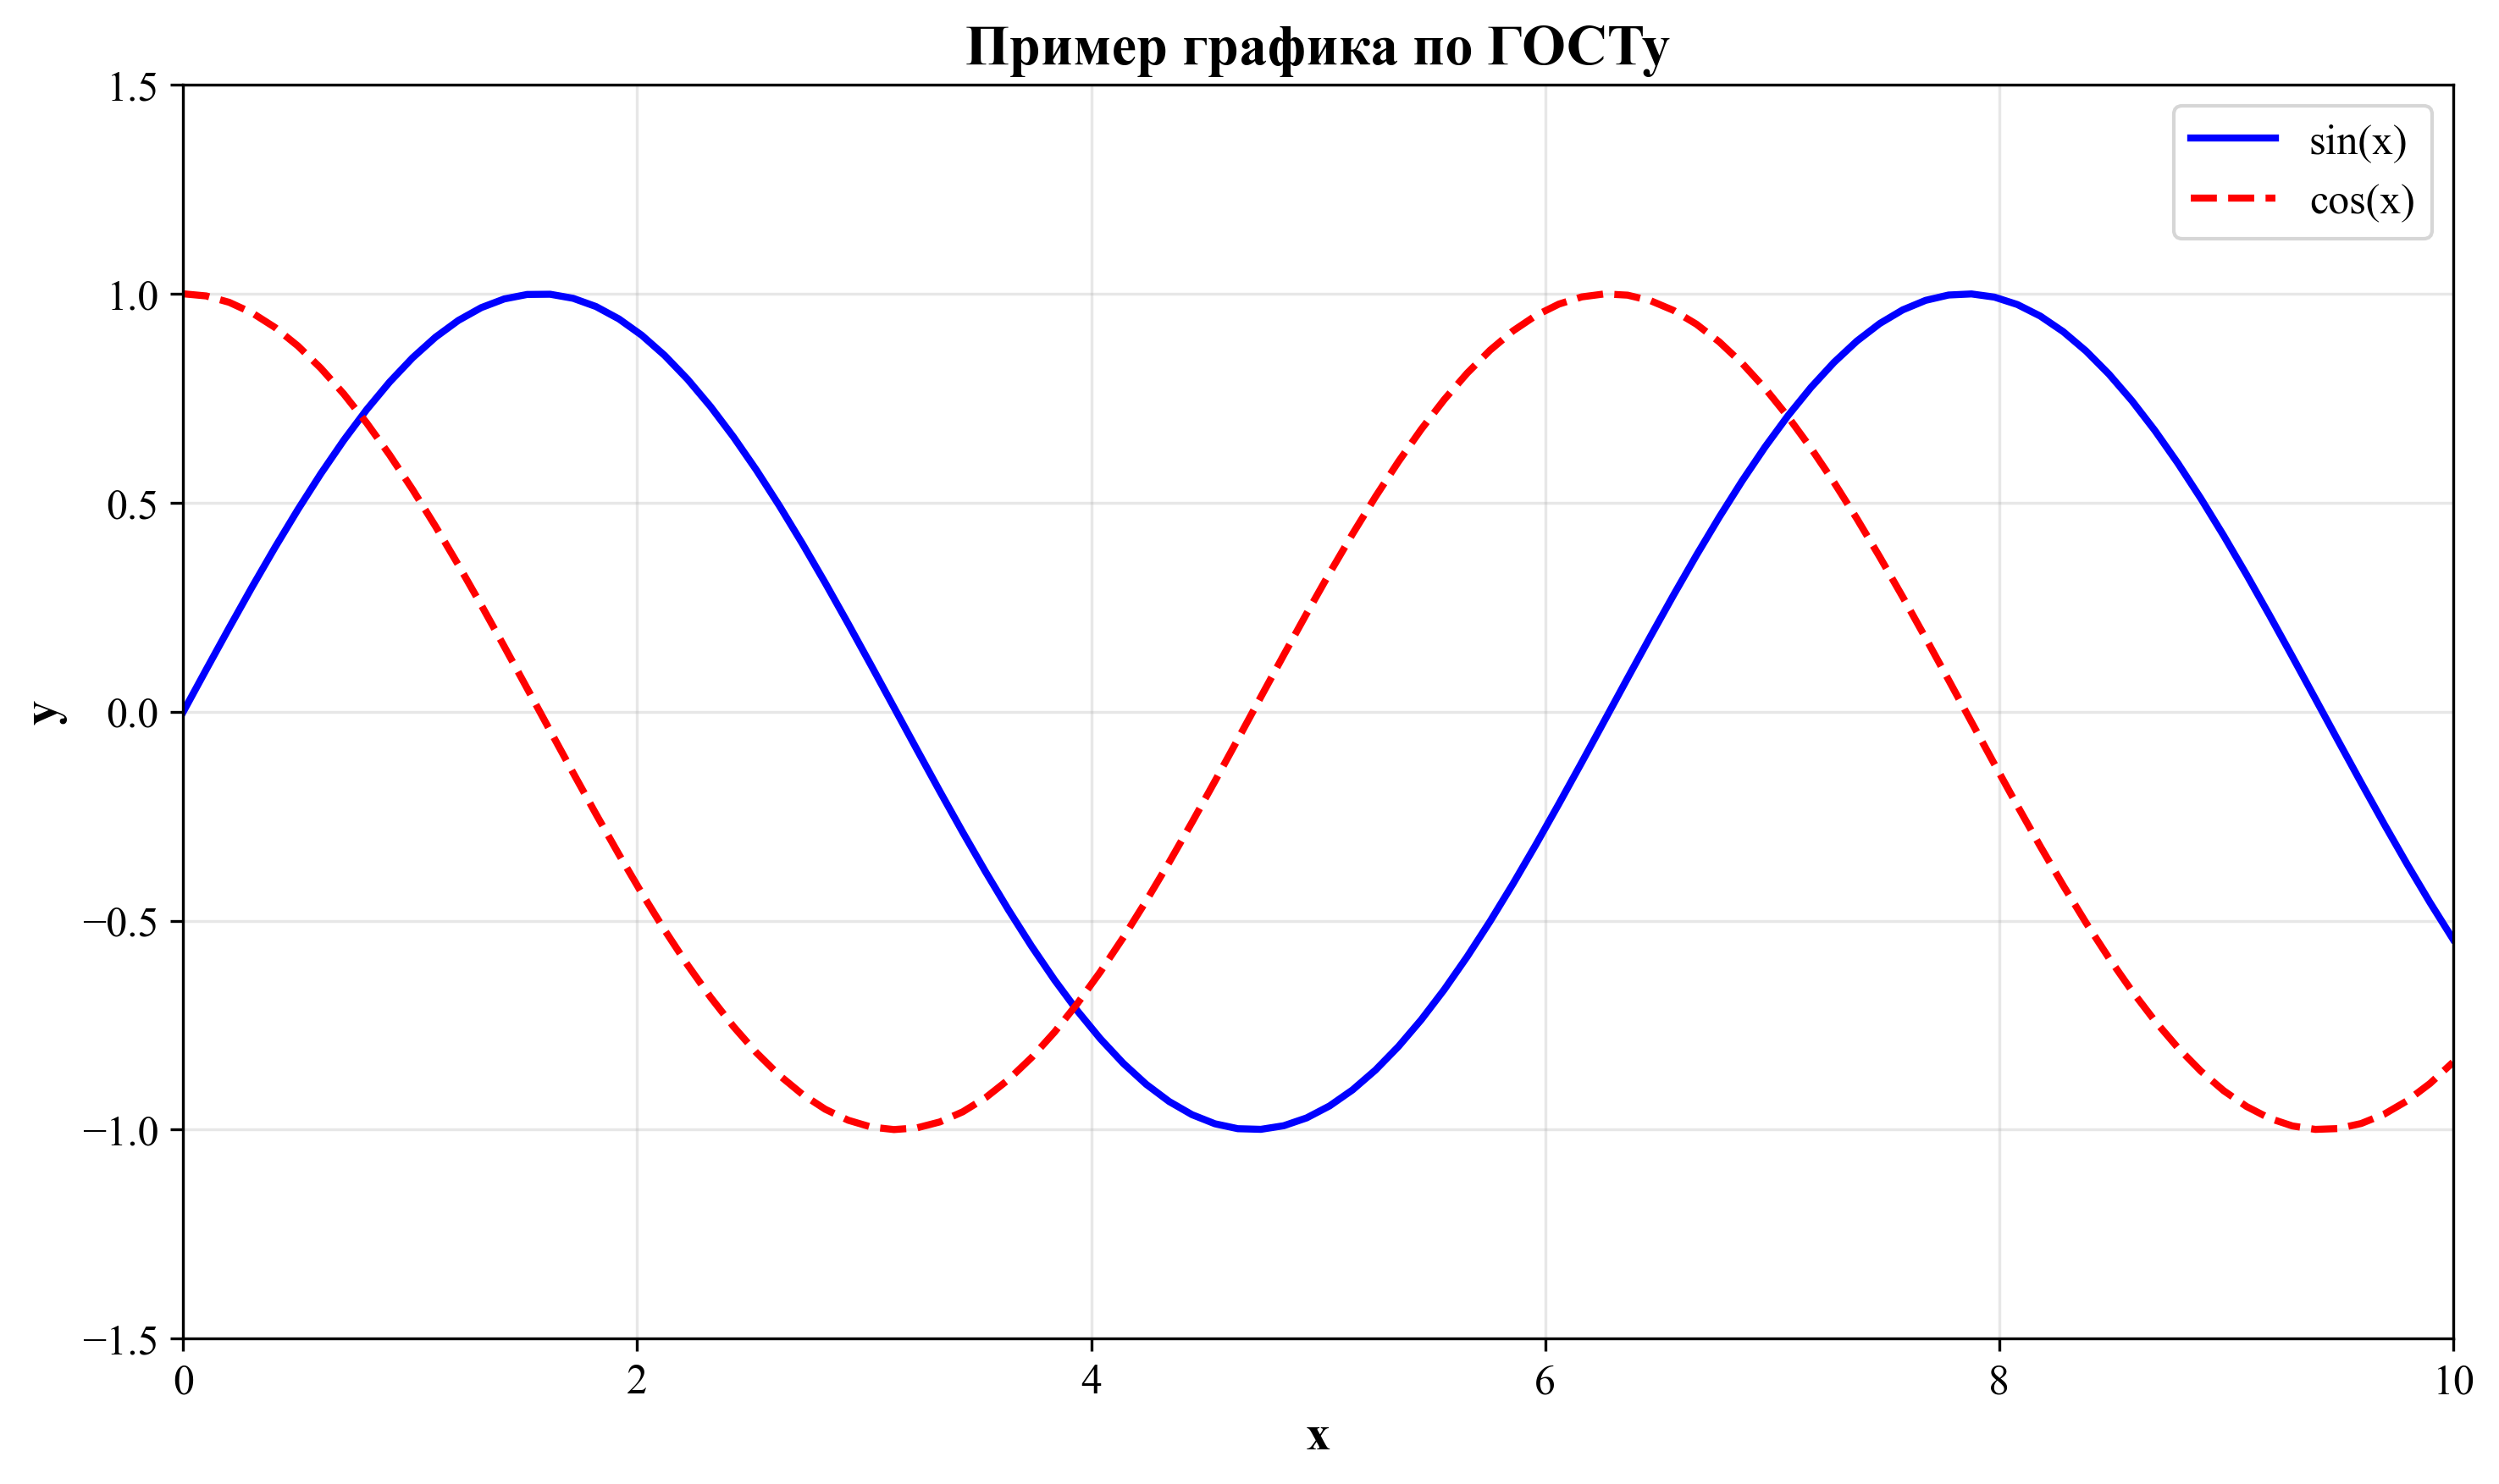
\includegraphics[width=0.8\textwidth]{images/example_plot.png}
\caption{График зависимости точности от размера выборки}
\label{fig:accuracy_plot}
\end{figure}

% Пример правильной вставки изображения по ГОСТу 7.32-2017
\begin{figure}[H]
\centering
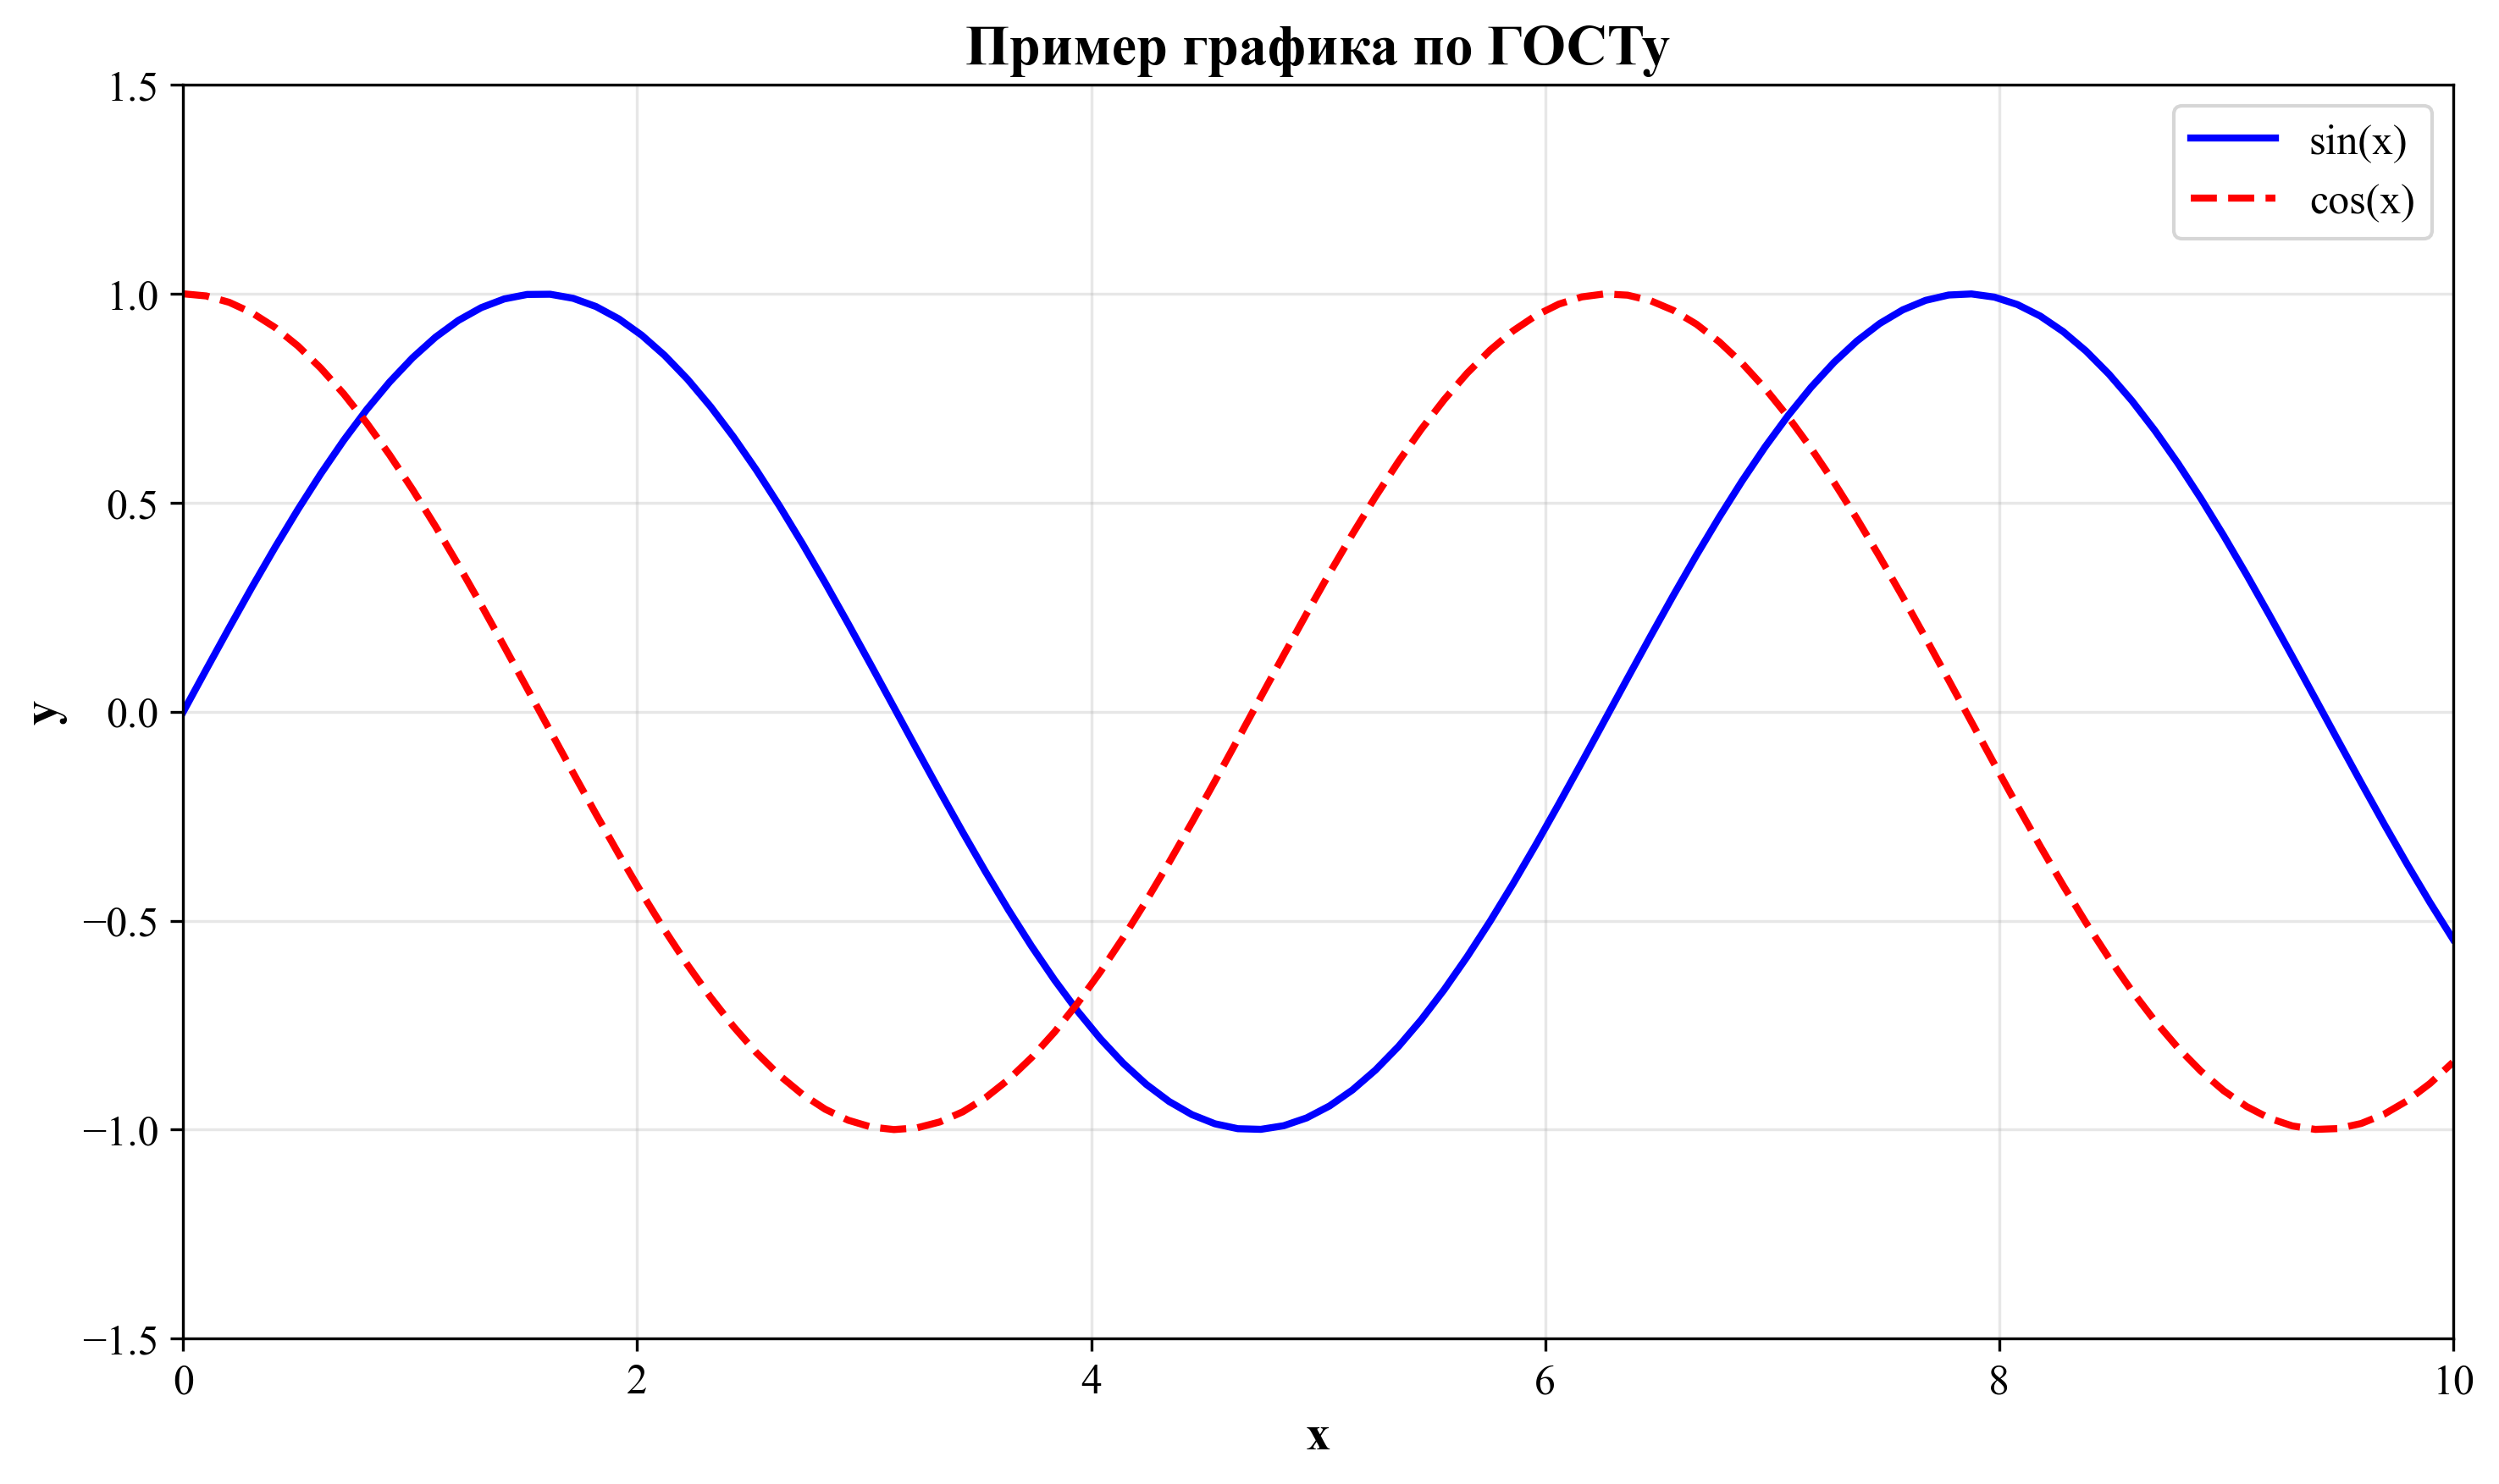
\includegraphics[width=0.6\textwidth]{images/example_plot.png}
\caption{Пример графика по ГОСТу: зависимость функций sin(x) и cos(x) от аргумента x}
\label{fig:gost_example}
\end{figure}

\section{Статистический анализ}

Результаты статистического анализа данных представлены в таблице~\ref{tab:statistics}.

\begin{table}[H]
\centering
\caption{Статистические показатели}
\begin{tabular}{|l|c|c|c|}
\hline
Показатель & Значение & Стандартное отклонение & Доверительный интервал \\
\hline
Среднее & 0.92 & 0.05 & [0.90, 0.94] \\
Медиана & 0.91 & - & - \\
Мода & 0.95 & - & - \\
\hline
\end{tabular}
\label{tab:statistics}
\end{table}

\note{Все значения округлены до двух знаков после запятой.}

\section{Примеры переноса таблиц и листингов}

\subsection{Перенос таблицы}

\begin{longtable}{|l|c|c|c|}
\caption{Длинная таблица с переносом страниц} \label{tab:long_table} \\
\hline
\textbf{№} & \textbf{Параметр} & \textbf{Значение} & \textbf{Результат} \\
\hline
\endfirsthead

\tablecontinuation{\thetable} \\
\hline
\textbf{№} & \textbf{Параметр} & \textbf{Значение} & \textbf{Результат} \\
\hline
\endhead

\hline
\endfoot

\hline
\endlastfoot

1 & A1 & 0.1 & 0.95 \\
2 & A2 & 0.2 & 0.87 \\
3 & A3 & 0.3 & 0.92 \\
4 & B1 & 0.4 & 0.88 \\
5 & B2 & 0.5 & 0.91 \\
6 & B3 & 0.6 & 0.89 \\
7 & C1 & 0.7 & 0.93 \\
8 & C2 & 0.8 & 0.86 \\
9 & C3 & 0.9 & 0.94 \\
10 & D1 & 1.0 & 0.90 \\
11 & A1 & 0.1 & 0.95 \\
12 & A2 & 0.2 & 0.87 \\
13 & A3 & 0.3 & 0.92 \\
14 & B1 & 0.4 & 0.88 \\
15 & B2 & 0.5 & 0.91 \\
16 & B3 & 0.6 & 0.89 \\
17 & C1 & 0.7 & 0.93 \\
18 & C2 & 0.8 & 0.86 \\
19 & C3 & 0.9 & 0.94 \\
20 & D1 & 1.0 & 0.90 \\
21 & A1 & 0.1 & 0.95 \\
22 & A2 & 0.2 & 0.87 \\
23 & A3 & 0.3 & 0.92 \\
24 & B1 & 0.4 & 0.88 \\
25 & B2 & 0.5 & 0.91 \\
26 & B3 & 0.6 & 0.89 \\
27 & C1 & 0.7 & 0.93 \\
28 & C2 & 0.8 & 0.86 \\
29 & C3 & 0.9 & 0.94 \\
30 & D1 & 1.0 & 0.90 \\

\end{longtable}

\subsection{Пример листинга кода}

\begin{lstlisting}[language=Python, caption={Пример алгоритма машинного обучения}, label={lst:ml_algorithm}, style=breakable]
import numpy as np
import pandas as pd
from sklearn.model_selection import train_test_split, cross_val_score
from sklearn.ensemble import RandomForestClassifier, GradientBoostingClassifier
from sklearn.svm import SVC
from sklearn.metrics import accuracy_score, classification_report
import matplotlib.pyplot as plt
import seaborn as sns

def preprocess_data(df):
    """Preprocess the dataset"""
    # Handle missing values
    df = df.fillna(df.mean())
    
    # Encode categorical variables
    categorical_columns = df.select_dtypes(include=['object']).columns
    for col in categorical_columns:
        df[col] = pd.Categorical(df[col]).codes
    
    return df

def train_model(X, y, model_type='random_forest'):
    """Train machine learning model"""
    # Split the data
    X_train, X_test, y_train, y_test = train_test_split(
        X, y, test_size=0.2, random_state=42, stratify=y
    )
    
    # Initialize model
    if model_type == 'random_forest':
        model = RandomForestClassifier(
            n_estimators=100,
            max_depth=10,
            random_state=42,
            n_jobs=-1
        )
    elif model_type == 'gradient_boosting':
        model = GradientBoostingClassifier(
            n_estimators=100,
            learning_rate=0.1,
            max_depth=6,
            random_state=42
        )
    elif model_type == 'svm':
        model = SVC(
            kernel='rbf',
            C=1.0,
            gamma='scale',
            random_state=42
        )
    else:
        raise ValueError("Unknown model type")
    
    # Train the model
    model.fit(X_train, y_train)
    
    # Make predictions
    y_pred = model.predict(X_test)
    
    # Calculate metrics
    accuracy = accuracy_score(y_test, y_pred)
    cv_scores = cross_val_score(model, X, y, cv=5, scoring='accuracy')
    
    # Print results
    print(f"Model: {model_type}")
    print(f"Accuracy: {accuracy:.4f}")
    print(f"CV Score: {cv_scores.mean():.4f} (+/- {cv_scores.std() * 2:.4f})")
    print("\nClassification Report:")
    print(classification_report(y_test, y_pred))
    
    return model, accuracy, y_pred

def plot_results(y_true, y_pred, model_name):
    """Plot classification results"""
    plt.figure(figsize=(10, 6))
    
    # Confusion matrix
    from sklearn.metrics import confusion_matrix
    cm = confusion_matrix(y_true, y_pred)
    
    plt.subplot(1, 2, 1)
    sns.heatmap(cm, annot=True, fmt='d', cmap='Blues')
    plt.title(f'Confusion Matrix - {model_name}')
    plt.xlabel('Predicted')
    plt.ylabel('Actual')
    
    # Feature importance (for tree-based models)
    plt.subplot(1, 2, 2)
    if hasattr(model, 'feature_importances_'):
        importances = model.feature_importances_
        indices = np.argsort(importances)[::-1][:10]
        plt.bar(range(10), importances[indices])
        plt.title(f'Feature Importance - {model_name}')
        plt.xlabel('Features')
        plt.ylabel('Importance')
    
    plt.tight_layout()
    plt.show()

# Example usage
if __name__ == "__main__":
    # Load data
    data = pd.read_csv('data.csv')
    
    # Preprocess
    data = preprocess_data(data)
    
    # Prepare features and target
    X = data.drop('target', axis=1)
    y = data['target']
    
    # Train different models
    models = ['random_forest', 'gradient_boosting', 'svm']
    results = {}
    
    for model_type in models:
        print(f"\n{'='*50}")
        print(f"Training {model_type}")
        print('='*50)
        
        model, accuracy, y_pred = train_model(X, y, model_type)
        results[model_type] = {
            'model': model,
            'accuracy': accuracy,
            'predictions': y_pred
        }
    
    # Compare results
    print("\n" + "="*50)
    print("MODEL COMPARISON")
    print("="*50)
    for model_name, result in results.items():
        print(f"{model_name}: {result['accuracy']:.4f}")
    
    # Plot results for best model
    best_model = max(results.items(), key=lambda x: x[1]['accuracy'])
    print(f"\nBest model: {best_model[0]} with accuracy {best_model[1]['accuracy']:.4f}")
\end{lstlisting}

\notes{
\item Все алгоритмы реализованы на языке Python версии 3.8+
\item Использованы библиотеки scikit-learn, numpy, pandas
\item Эксперименты проводились на сервере с 16 ГБ RAM
}
